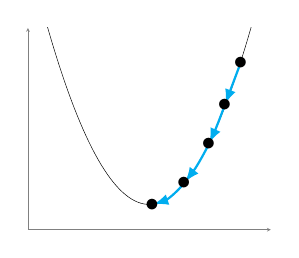
\begin{tikzpicture}[scale=.45]
        \begin{axis}[   
            grid=minor,  
            ticks=none,
            xmin=0,
            xmax=4,
            axis x line=bottom,
            ymax=.8,
            ymin=0,
            axis y line=left,
            no markers,
            axis line style=gray,
            xlabel style=gray,
            ylabel style=gray
        ]
            \addplot[black,mark=none,samples=200,domain=0:10,] (x,{(x/2-1)^2+.1});
            %\addplot[dashed,black,mark=none,samples=200,domain=0:10,] (x,{.7*x-1.8});
        \end{axis}
        
        \node[inner sep=-.2mm] (A) at (6,4.7){};
        \node[inner sep=-.2mm] (B) at (5.55,3.5){};
        \node[inner sep=-.2mm] (C) at (5.1,2.4){};
        \node[inner sep=-.2mm] (D) at (4.4,1.3){};
        \node[inner sep=-.2mm] (E) at (3.5,.7){};
        
        \draw[-latex,cyan, thick] (A) -- (B);
        \draw[-latex,cyan, thick] (B) edge[bend left=2] (C);
        \draw[-latex,cyan, thick] (C) edge[bend left=5] (D);
        \draw[-latex,cyan, thick] (D) edge[bend left=15] (E);
        
        \node[inner sep=-.2mm] at (A){$\bullet$};
        \node[inner sep=-.2mm] at (B){$\bullet$};
        \node[inner sep=-.2mm] at (C){$\bullet$};
        \node[inner sep=-.2mm] at (D){$\bullet$};
        \node[inner sep=-.2mm] at (E){$\bullet$};
        
	\end{tikzpicture}